\documentclass[a4paper,11pt,reqno]{amsart}

\usepackage[T1]{fontenc}
\usepackage{lmodern}
\usepackage{microtype}
\usepackage[a4paper,left=24mm,right=24mm,top=22mm,bottom=24mm]{geometry}
\usepackage{mathtools,amssymb,amsthm}
\usepackage{xcolor}
\definecolor{linkviolet}{RGB}{112,60,160}
\definecolor{citeblue}{RGB}{35,82,145}
\usepackage{tikz}
\usepackage{quiver}
\usepackage[shortlabels]{enumitem}
\usepackage{needspace}
\usepackage{hyperref}

\newtheorem{maintheorem}{Theorem}
\renewcommand{\themaintheorem}{\Alph{maintheorem}}
\newtheorem{maincorollary}[maintheorem]{Corollary}
\newtheorem{theorem}{Theorem}[section]
\newtheorem{proposition}[theorem]{Proposition}
\newtheorem{lemma}[theorem]{Lemma}
\newtheorem{corollary}[theorem]{Corollary}
\theoremstyle{definition}
\newtheorem{definition}[theorem]{Definition}
\newtheorem{example}[theorem]{Example}
\newtheorem{remark}[theorem]{Remark}

\newcommand{\Z}{\mathbb Z}
\newcommand{\Q}{\mathbb Q}
\newcommand{\D}{\Q/\Z}
\newcommand{\U}{\operatorname U}
\newcommand{\Sym}{\operatorname{Sym}}
\newcommand{\gr}{\operatorname{gr}}
\newcommand{\ab}{\operatorname{ab}}

\newcommand{\presentationlangle}{%
  \mathopen{\vcenter{\hbox{%
    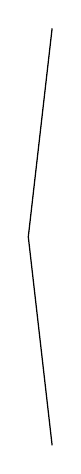
\begin{tikzpicture}[x=1ex,y=1ex,baseline=(current bounding box.center)]
      \draw[line width=.45pt] (2,17.5) -- (0,0) -- (2,-17.5);
    \end{tikzpicture}%
  }}}%
}
\newcommand{\presentationrangle}{%
  \mathclose{\vcenter{\hbox{%
    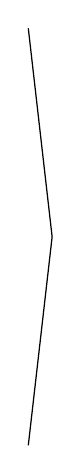
\begin{tikzpicture}[x=1ex,y=1ex,baseline=(current bounding box.center)]
      \draw[line width=.45pt] (0,17.5) -- (2,0) -- (0,-17.5);
    \end{tikzpicture}%
  }}}%
}

\title{Some Results on Dimension Subrings in Lie Rings}
\author{Vasily Ionin}
\author{Roman Mikhailov}
\author{Tima Petrov}
\date{}

\hypersetup{
  colorlinks=true,
  linkcolor=linkviolet,
  citecolor=citeblue,
  urlcolor=citeblue,
  pdftitle={Some Results on Dimension Subrings in Lie Rings},
  pdfauthor={Vasily Ionin, Roman Mikhailov, and Tima Petrov}
}

\subjclass[2020]{17B35, 17B30, 20C05}
\keywords{Lie ring, dimension subring, lower central series, universal
enveloping algebra, metabelian Lie ring}

\begin{document}

\maketitle

\section{Introduction}

Let $G$ be a group.  Its lower central series is defined by
\[
 \gamma _1(G)=G,
 \qquad
 \gamma _{n+1}(G)=[\gamma _n(G),G].
\]
Let $\Delta(G)$ denote the augmentation ideal of the integral group ring
$\Z[G]$.  The dimension subgroups of $G$ are
\[
 D_n(G)=G\cap\bigl(1+\Delta(G)^n\bigr)
       =\{g\in G\mid g-1\in\Delta(G)^n\}.
\]
The commutator identity in $\Z[G]$ gives
$\gamma_n(G)\subseteq D_n(G)$ for every $n$.  The equality
$D_n(G)=\gamma_n(G)$ holds for $n\leq 3$, but fails in general: Rips
constructed a group for which $D_4(G)\neq\gamma_4(G)$~\cite{Rips1972}.
The free-group and free-Lie-ring cases are due to Magnus
and Witt, respectively~\cite{Magnus1937,Witt1937}.  We refer
to~\cite{Passi1979,MikhailovPassi2009} for the classical dimension-subgroup
problem and its subsequent development.

There is a parallel theory for Lie rings.  For a Lie ring $L$, let $\U(L)$
be its universal enveloping algebra and let $\varpi(L)$ be the kernel of the
augmentation $\U(L)\to\Z$.  The lower central series and the dimension
series of $L$ are
\[
 \gamma_1(L)=L,
 \qquad
 \gamma_{n+1}(L)=[\gamma_n(L),L],
 \qquad
 \delta_n(L)=L\cap\varpi(L)^n.
\]
Here and below $L$ is identified with its image in $\U(L)$; this is valid
over $\Z$ by the integral Birkhoff--Witt theorem.  As in the group case,
\[
                     \gamma_n(L)\subseteq\delta_n(L).
\]
Bartholdi and Passi proved that
$\delta_n(L)=\gamma_n(L)$ for $n\leq3$ and constructed a Lie-ring analogue
of the Rips example in degree four~\cite{BartholdiPassi2015}.

\subsection{No stabilization for dimension series}

The lower central series has an elementary stabilization property: if
$\gamma_m(L)=\gamma_{m+1}(L)$, then $\gamma_q(L)=\gamma_m(L)$ for every
$q\geq m$.  The analogous statement fails for the dimension series:
arbitrarily many consecutive terms may coincide without subsequent
stabilization.

\Needspace{9\baselineskip}
\begin{maintheorem}\label{thm:A}
For every integer $N\geq1$, there exist an integer $m=m(N)\geq1$ and a Lie
ring $L_N$ such that
\[
 \delta_m(L_N)=\delta_{m+1}(L_N)=\cdots=\delta_{m+N}(L_N)
 \neq\delta_{m+N+1}(L_N).
\]
\end{maintheorem}

An explicit construction of $L_N$ is given in
Section~\ref{sec:plateaux}.  In this construction, $m(N)=N+4$, and $L_N$
is metabelian and nilpotent of class $N+3$.

\subsection{Centrality of dimension series}

Gupta and Kuz'min proved that, for every group $G$ and every $n\geq1$,
$D_n(G)/\gamma_{n+1}(G)$ is abelian~\cite{GuptaKuzmin1992}; equivalently,
\[
                    [D_n(G),D_n(G)]\subseteq\gamma_{n+1}(G).
\]
Bartholdi and Passi proved that
$\delta_n(L)/\gamma_{n+1}(L)$ is abelian for every Lie ring
$L$~\cite{BartholdiPassi2015}.  Gupta and Kuz'min also proved that
\[
                         [D_4(G),G]=\gamma_5(G)
\]
for every group $G$~\cite{GuptaKuzmin1992}.  For general $n$, however,
$D_n(G)/\gamma_{n+1}(G)$ need not be central in
$G/\gamma_{n+1}(G)$~\cite{GuptaKuzmin1995}.  Passi and Sicking proved
that
\[
                         [\delta_n(L),L]=\gamma_{n+1}(L)
\]
for every metabelian Lie ring $L$~\cite{PassiSicking2017}.  For a Lie
algebra over a commutative ring $k$, define $\delta_n(L)$ as
the inverse image of $\varpi_k(L)^n$ under the canonical map
$L\to\U_k(L)$.  The following theorem shows that the metabelian hypothesis
is unnecessary.

\begin{maintheorem}\label{thm:B}
Let $L$ be a Lie algebra over a commutative ring with identity.  For all
$m,n\geq1$,
\[
                 [\delta_n(L),\delta_m(L)]\subseteq\gamma_{n+m}(L).
\]
In particular,
\[
                       [\delta_n(L),L]=\gamma_{n+1}(L).
\]
\end{maintheorem}

\subsection{Plotkin's problem for metabelian Lie rings}

We prove a uniform vanishing bound for metabelian nilpotent Lie rings.

\begin{maintheorem}\label{thm:C}
Let $c\geq2$.  If $L$ is a metabelian Lie ring of nilpotency class at most
$c$, then
\[
                              \delta_{2c-1}(L)=0.
\]
\end{maintheorem}

Theorem~\ref{thm:C} shows that the construction in Theorem~\ref{thm:A} is
optimal with respect to the nilpotency class: every metabelian Lie ring
$L$ of nilpotency class at most $N+3$ satisfies
\[
             \delta_{m(N)+N+1}(L)=0,
             \qquad m(N)=N+4.
\]

\begin{maincorollary}\label{cor:D}
For every Lie ring $L$ and every $c\geq2$,
\[
              \delta_{2c-1}(L)\subseteq\gamma_{c+1}(L)+L''.
\]
In particular, $\delta_5(L)\subseteq\gamma_4(L)$.
\end{maincorollary}

The corresponding question for groups remains open: is
$D_5(G)\subseteq\gamma_4(G)$ for every group $G$?
See~\cite[Problem~20.84]{KourovkaNotebook20}.

For a group $G$, put
\[
 D_\omega(G)=\bigcap_{n\geq1}D_n(G),
 \qquad
 \gamma_\omega(G)=\bigcap_{n\geq1}\gamma_n(G).
\]
Plotkin asked whether $D_\omega(G)=\gamma_\omega(G)$ for every group
$G$~\cite{Plotkin1973}.  Our result gives an affirmative answer to the
Lie-ring analogue of Plotkin's problem for metabelian Lie rings.  For a
Lie ring $L$, define analogously
\[
 \delta_\omega(L)=\bigcap_{n\geq1}\delta_n(L),
 \qquad
 \gamma_\omega(L)=\bigcap_{n\geq1}\gamma_n(L).
\]

\begin{maincorollary}\label{cor:E}
If $L$ is a metabelian Lie ring, then
\[
              \delta_{2c-1}(L)\subseteq\gamma_{c+1}(L),
              \qquad c\geq2.
\]
In particular, $\delta_\omega(L)=\gamma_\omega(L)$.
\end{maincorollary}

\subsection{Organization}

Section~\ref{sec:preliminaries} records the integral PBW theorem and the
filtrations used below.  Sections~\ref{sec:plateaux},~\ref{sec:centrality},
and~\ref{sec:vanishing} prove
Theorems~\ref{thm:A},~\ref{thm:B}, and~\ref{thm:C}, respectively.
Section~\ref{sec:formalization} describes their verification in Lean~4.

\section{Preliminaries}\label{sec:preliminaries}

All commutators are left-normed:
\[
 [x_1,x_2,\ldots,x_r]=[[\cdots[[x_1,x_2],x_3],\ldots],x_r].
\]
For additive subgroups $B_1,\ldots,B_r$ of a Lie ring, the notation
$[B_1,\ldots,B_r]$ denotes the subgroup generated by the corresponding
commutators.  For an ideal $A$ of $L$, set
\[
 [A,{}_0L]=A,
 \qquad
 [A,{}_{r+1}L]=[[A,{}_rL],L].
\]
A Lie ring $L$ is metabelian if
$L''=[[L,L],[L,L]]=0$.

\subsection{The integral PBW theorem}

Let $T(L)=\bigoplus_{r\geq0}L^{\otimes r}$ be the tensor algebra of the
underlying abelian group of $L$.  The universal enveloping algebra is
\[
 \U(L)=T(L)/\bigl(x\otimes y-y\otimes x-[x,y]\mid x,y\in L\bigr).
\]
The tensor-length filtration induces the increasing PBW filtration
\[
 P_0\U(L)\subseteq P_1\U(L)\subseteq P_2\U(L)\subseteq\cdots,
\]
where $P_r\U(L)$ is generated additively by products of at most $r$
elements of $L$.

\begin{theorem}\label{thm:PBW}
For every Lie ring $L$, the canonical maps
\[
 L\longrightarrow\U(L),
 \qquad
 \Sym_{\Z}(L)\longrightarrow\gr_P\U(L)
\]
are, respectively, injective and an isomorphism of graded algebras.
\end{theorem}

This is the Birkhoff--Witt theorem over the Dedekind domain $\Z$; see
Higgins~\cite{Higgins1969}.  We use the following explicit consequence.

\begin{corollary}\label{cor:PBW-collection}
Suppose that the additive group of $L$ has an ordered decomposition
\[
 L=\bigoplus_{i\in I}\langle x_i\rangle,
\]
where each summand is cyclic, finite or infinite.  Then
the following statements hold.
\begin{enumerate}[(i)]
 \item For every $r\geq1$, the quotient
 $P_r\U(L)/P_{r-1}\U(L)$ is the direct sum of the cyclic groups generated
 by the ordered products
 \[
  x_{i_1}\cdots x_{i_r},
                         \qquad i_1\leq\cdots\leq i_r.
 \]
 The additive order of such a generator is the greatest common divisor of
 the additive orders of its factors, with order zero interpreted as
 infinite.
 \item For $r\geq1$, let $M_r$ be the subgroup of $\U(L)$ generated by
 the ordered products of length $r$, and put $M_0=\Z\cdot1$.  Then
 \[
  P_r\U(L)=\bigoplus_{q=0}^r M_q,
  \qquad
  \U(L)=\bigoplus_{q\geq0}M_q.
 \]
 Consequently, for every $s\geq0$, the rule
 \[
  p_{\leq s}(x_{i_1}\cdots x_{i_r})=
  \begin{cases}
   x_{i_1}\cdots x_{i_r},&r\leq s,\\
   0,&r>s,
  \end{cases}
  \qquad i_1\leq\cdots\leq i_r,
 \]
 defines an additive retraction
 \[
                     p_{\leq s}:\U(L)\longrightarrow P_s\U(L).
 \]
\end{enumerate}
\end{corollary}

\begin{proof}
By Theorem~\ref{thm:PBW}, the quotient in (i) is $\Sym^r_{\Z}(L)$.
Thus (i) follows by taking symmetric powers of the given direct sum.

For (ii), part (i) shows that the map
\[
                      M_r\longrightarrow P_r\U(L)/P_{r-1}\U(L)
\]
is surjective.  If an element of $M_r$ maps to zero, the coefficient of
each ordered product is divisible by the additive order of its image in
the quotient.  If this order is zero, the coefficient is zero.  Otherwise,
let $d_j$ be the additive order of $x_{i_j}$, with $d_j=0$ for infinite
order, and set $d=\gcd(d_1,\ldots,d_r)$.  By (i), $d$ is the order of the
image of $x_{i_1}\cdots x_{i_r}$.  Each $d_j$ annihilates this product, so
B\'ezout's identity implies that $d$ also annihilates it.  Therefore the
map is injective, and
$P_r\U(L)=P_{r-1}\U(L)\oplus M_r$.  Induction on $r$ proves both
decompositions and the assertion about $p_{\leq s}$.
\end{proof}

The augmentation $\U(L)\to\Z$ is induced by the zero map $L\to\Z$.  Its
kernel $\varpi(L)$ is the two-sided ideal generated by $L$.  Thus
$\varpi(L)^n$ is generated additively by products of at least $n$ elements
of $L$.

\subsection{Dimension subrings}

For every $n\geq1$,
\begin{equation}\label{eq:lower-in-dimension}
                         \gamma_n(L)\subseteq\delta_n(L).
\end{equation}
Indeed, $L\subseteq\varpi(L)$ and
$[\varpi(L)^r,\varpi(L)]\subseteq\varpi(L)^{r+1}$, so
\eqref{eq:lower-in-dimension} follows by induction.  Both series are
functorial: a homomorphism $f:L\to M$ satisfies
\[
 f(\gamma_n(L))\subseteq\gamma_n(M),
 \qquad
 f(\delta_n(L))\subseteq\delta_n(M).
\]

We also use the following result of Passi and Sicking.

\begin{theorem}\label{thm:Passi-Sicking}
If $L$ is metabelian, then, for every $n\geq1$,
\[
             2\delta_n(L)\subseteq\gamma_n(L).
\]
\end{theorem}

This is~\cite[Theorem~1.1]{PassiSicking2017}.

\section{Finite plateaux}\label{sec:plateaux}

Fix an integer $N\geq1$.  Let $F$ be the free metabelian Lie ring on
$x_1,\ldots,x_5$.  Order the generators by
\[
                         x_5<x_1<x_2<x_3<x_4.
\]
The standard metabelian Hall basis consists of the generators and the
commutators
\[
 [x_{i_0},x_{i_1},\ldots,x_{i_r}],
 \qquad
 x_{i_0}>x_{i_1}\leq x_{i_2}\leq\cdots\leq x_{i_r}.
\]
Put
\[
 t=[x_4,\underbrace{x_5,\ldots,x_5}_{N}],
 \qquad
 c_i=[t,x_i],
 \qquad
 u_i=[c_i,x_i],
 \quad 1\leq i\leq3.
\]
Thus $t$, $c_i$, and $u_i$ have weights $N+1$, $N+2$, and $N+3$,
respectively.  With the chosen order, the three $u_i$ are distinct Hall
basis elements.

Define the relators
\begin{equation}\label{eq:shifted-relators}
 \begin{aligned}
 r_1&=4x_1+2c_3+c_2,\\
 r_2&=16x_2+4c_3-c_1,\\
 r_3&=64x_3-4c_2-2c_1.
 \end{aligned}
\end{equation}
Let $L_N$ be the quotient of $F$ by the Lie ideal specified as follows:
\begin{enumerate}[(i)]
 \item impose $r_1=r_2=r_3=0$;
 \item factor out $\gamma_{N+4}(F)$;
 \item in weight $N+3$, factor out all Hall basis elements other than
 $u_1,u_2,u_3$;
 \item impose
 \[
                    u_1=16u_3,
                    \qquad u_2=4u_3,
                    \qquad 64u_3=0.
 \]
\end{enumerate}

\begin{example}\label{ex:first-two-plateaux}
Let $\mathcal H_q$ denote the weight-$q$ part of the metabelian Hall basis
fixed above.  A subscript $\mathrm{met}$ indicates a presentation in the
variety of metabelian Lie rings.  Substituting $N=1$ gives
\[
\begin{aligned}
L_1={}&
\presentationlangle
\left.
x_1,x_2,x_3,x_4,x_5
\ \middle|\
\begin{aligned}
\text{(i)}\;&\quad
 \begin{gathered}
 4x_1+2[x_4,x_5,x_3]+[x_4,x_5,x_2]=0,\\
 16x_2+4[x_4,x_5,x_3]-[x_4,x_5,x_1]=0,\\
 64x_3-4[x_4,x_5,x_2]-2[x_4,x_5,x_1]=0;
 \end{gathered}\\[5pt]
\text{(ii)}\;&\quad \gamma_5=0;\\[5pt]
\text{(iii)}\;&\quad
 \begin{gathered}
 h=0\quad\text{for }h\in\mathcal H_4\setminus
 \{[x_4,x_5,x_1,x_1],\\
 \hfill [x_4,x_5,x_2,x_2],[x_4,x_5,x_3,x_3]\};
 \end{gathered}\\[5pt]
\text{(iv)}\;&\quad
 \begin{gathered}
 [x_4,x_5,x_1,x_1]=16[x_4,x_5,x_3,x_3],\\
 [x_4,x_5,x_2,x_2]=4[x_4,x_5,x_3,x_3],\\
 64[x_4,x_5,x_3,x_3]=0.
\end{gathered}
\end{aligned}
\right.
\presentationrangle_{\mathrm{met}}.
\end{aligned}
\]
Similarly,
\[
\begin{aligned}
L_2={}&
\presentationlangle
\left.
x_1,x_2,x_3,x_4,x_5
\ \middle|\
\begin{aligned}
\text{(i)}\;&\quad
 \begin{gathered}
 4x_1+2[x_4,x_5,x_5,x_3]+[x_4,x_5,x_5,x_2]=0,\\
 16x_2+4[x_4,x_5,x_5,x_3]-[x_4,x_5,x_5,x_1]=0,\\
 64x_3-4[x_4,x_5,x_5,x_2]-2[x_4,x_5,x_5,x_1]=0;
 \end{gathered}\\[5pt]
\text{(ii)}\;&\quad \gamma_6=0;\\[5pt]
\text{(iii)}\;&\quad
 \begin{gathered}
 h=0\quad\text{for }h\in\mathcal H_5\setminus
 \{[x_4,x_5,x_5,x_1,x_1],\\
 \hfill [x_4,x_5,x_5,x_2,x_2],[x_4,x_5,x_5,x_3,x_3]\};
 \end{gathered}\\[5pt]
\text{(iv)}\;&\quad
 \begin{gathered}
 [x_4,x_5,x_5,x_1,x_1]=16[x_4,x_5,x_5,x_3,x_3],\\
 [x_4,x_5,x_5,x_2,x_2]=4[x_4,x_5,x_5,x_3,x_3],\\
 64[x_4,x_5,x_5,x_3,x_3]=0.
\end{gathered}
\end{aligned}
\right.
\presentationrangle_{\mathrm{met}}.
\end{aligned}
\]
\end{example}

\begin{lemma}\label{lem:top-layer}
The Lie ring $L_N$ is metabelian and nilpotent of class $N+3$, and
\[
             \gamma_{N+3}(L_N)=\langle u_3\rangle\cong\Z/64.
\]
\end{lemma}

\begin{proof}
Metabelianity is inherited from $F$, and relation (ii) gives
$\gamma_{N+4}(L_N)=0$.  By relation~\textup{(iii)},
$\gamma_{N+3}(L_N)$ is generated by $u_1,u_2,u_3$.  Hall collection shows
that the induced relations are precisely those in~\textup{(iv)}, with
matrix
\[
 \begin{pmatrix}
  1&0&-16\\
  0&1&-4\\
  0&0&64
 \end{pmatrix}.
\]
Its Smith reduction gives a cyclic quotient of order $64$, generated by
$u_3$.  Thus $\gamma_{N+3}(L_N)\neq0$, while
$\gamma_{N+4}(L_N)=0$.
\end{proof}

Set
\[
 b_{12}=[x_1,x_2],
 \qquad
 b_{13}=[x_1,x_3],
 \qquad
 b_{23}=[x_2,x_3]
\]
and define
\begin{equation}\label{eq:a-definition}
                 a=32b_{12}+64b_{13}+128b_{23}\in L_N.
\end{equation}

Bracketing the relators~\eqref{eq:shifted-relators} with $x_1,x_2,x_3$ and
using $[F',F']=0$ together with relation~\textup{(iii)} gives
\begin{equation}\label{eq:six-relations}
 \begin{array}{rclrcl}
 4b_{12}+u_2&=&0,& 4b_{13}+2u_3&=&0,\\
 -16b_{12}-u_1&=&0,&16b_{23}+4u_3&=&0,\\
 -64b_{13}-2u_1&=&0,&-64b_{23}-4u_2&=&0.
 \end{array}
\end{equation}

\begin{lemma}\label{lem:a-order}
In $L_N$ one has $a=32u_3$.  In particular,
\[
                         \langle a\rangle\cong\Z/2.
\]
\end{lemma}

\begin{proof}
Three relations in~\eqref{eq:six-relations} give
\[
 32b_{12}=-2u_1,
 \qquad
 64b_{13}=-2u_1,
 \qquad
 128b_{23}=-8u_2.
\]
Since $u_1=16u_3$, $u_2=4u_3$, and $64u_3=0$, it follows that
\[
 a=-4u_1-8u_2=-96u_3=32u_3.
\]
By Lemma~\ref{lem:top-layer}, the element $u_3$ has order $64$; hence
$32u_3$ has order $2$.
\end{proof}

\begin{lemma}\label{lem:a-height}
The element $a$ belongs to $\delta_{2N+4}(L_N)$.
\end{lemma}

\begin{proof}
In $\U(L_N)$, expand~\eqref{eq:a-definition} as
\[
 a=x_1w_1+x_2w_2+x_3w_3,
\]
where
\[
 w_1=32x_2+64x_3,
 \qquad
 w_2=-32x_1+128x_3,
 \qquad
 w_3=-64x_1-128x_2.
\]
Since $t,c_i\in F'$ and $F$ is metabelian, $[t,c_i]=0$.  Bracketing the
relators~\eqref{eq:shifted-relators} with $t$ gives
\[
 4c_1=0,
 \qquad
 16c_2=0,
 \qquad
 64c_3=0.
\]
Together with the relators themselves, these identities give
\[
 w_1=4(c_1+c_2-2c_3),
 \qquad
 w_2=16(c_2+c_3),
 \qquad
 w_3=64c_3.
\]
Substitution from~\eqref{eq:shifted-relators} gives
\[
 4x_1=-(2c_3+c_2),
 \qquad
 16x_2=-(4c_3-c_1),
 \qquad
 64x_3=4c_2+2c_1.
\]
The elements $c_1,c_2,c_3$ lie in the abelian derived ring and therefore
commute in $\U(L_N)$.  Substituting the preceding identities gives
\begin{equation}\label{eq:a-factorization}
 \begin{aligned}
 a={}&(4x_1)(c_1+c_2-2c_3)
      +(16x_2)(c_2+c_3)+(64x_3)c_3\\
   ={}&c_1c_3-c_2^2.
 \end{aligned}
\end{equation}
Since $c_i\in\gamma_{N+2}(L_N)\subseteq\varpi(L_N)^{N+2}$,
equation~\eqref{eq:a-factorization} implies
$a\in\varpi(L_N)^{2N+4}$.
\end{proof}

\begin{lemma}\label{lem:critical-normal-form}
\[
                         L_N\cap\varpi(L_N)^{N+4}=\langle a\rangle.
\]
\end{lemma}

\begin{proof}
Let $z\in L_N\cap\varpi(L_N)^{N+4}$.  Since
$\gamma_{N+4}(L_N)=0$, Theorem~\ref{thm:Passi-Sicking} gives $2z=0$.
Theorem~\ref{thm:B} also gives $[z,L_N]=\gamma_{N+5}(L_N)=0$.  Express $z$
in the fixed metabelian Hall basis and apply PBW collection to its image in
$\U(L_N)$.
In degrees below $N+4$, the Hall elements of weights $3,\ldots,N+2$ have
distinct leading PBW monomials, so their coefficients vanish.  The
weight-two components of the equations $[z,x_i]=0$, together
with~\eqref{eq:shifted-relators}, leave only a linear combination of
\[
                         b_{12},\quad b_{13},\quad b_{23}
\]
together with $u_3$.

After substituting $u_1=16u_3$ and $u_2=4u_3$
into~\eqref{eq:six-relations} and discarding redundant relations, a relation
matrix for these four terms, with columns ordered as
$(b_{12},b_{13},b_{23},u_3)$, is
\begin{equation}\label{eq:critical-matrix}
 \begin{pmatrix}
  4&0&0&4\\
  0&4&0&2\\
  0&0&16&4\\
  0&0&0&64
 \end{pmatrix}.
\end{equation}
Let
\[
                 v=\alpha b_{12}+\beta b_{13}+\chi b_{23}+\eta u_3.
\]
Corollary~\ref{cor:PBW-collection}, applied in degrees $2$ and $N+3$, shows
that $v$ has trivial image in $\U(L_N)/\varpi(L_N)^{N+4}$ precisely when
\[
 \alpha\equiv0\pmod4,
 \qquad
 \beta\equiv0\pmod4,
 \qquad
 \chi\equiv0\pmod{16},
\]
and
\[
             \eta-\alpha-\frac{\beta}{2}-\frac{\chi}{4}
             \equiv0\pmod{32}.
\]
Under the first three congruences,~\eqref{eq:critical-matrix} gives
\[
 v=\left(\eta-\alpha-\frac{\beta}{2}-\frac{\chi}{4}\right)u_3.
\]
Thus the kernel is generated by $32u_3=a$, and it has order two by
Lemma~\ref{lem:a-order}.
\end{proof}

\begin{lemma}\label{lem:last-initial-form}
The element $a$ does not belong to $\varpi(L_N)^{2N+5}$.
\end{lemma}

\begin{proof}
Consider the augmentation-graded algebra
\[
 \gr_{\varpi}\U(L_N)
   =\bigoplus_{q\geq0}\varpi(L_N)^q/\varpi(L_N)^{q+1}.
\]
By~\eqref{eq:a-factorization}, the initial form of $a$ in degree $2N+4$
is
\[
                         \overline c_1\overline c_3-\overline c_2^2.
\]
The initial forms of the defining relators give
\[
                    4\overline c_1=0,
                    \qquad16\overline c_2=0,
                    \qquad64\overline c_3=0.
\]
Choose the PBW order so that
$\overline c_1\overline c_3$ is an ordered monomial.  PBW collection in
degree $2N+4$ shows that every relation in this graded component has even
coefficient at $\overline c_1\overline c_3$.
Therefore the rule
\[
 \varepsilon(\overline c_1\overline c_3)=1,
 \qquad
 \varepsilon(M)=0
 \quad\text{for every other ordered PBW monomial $M$ of this degree}
\]
is well defined and gives a homomorphism
\[
 \varepsilon:\varpi(L_N)^{2N+4}/\varpi(L_N)^{2N+5}
              \longrightarrow\Z/2.
\]
It sends the initial form of $a$ to $1$.  That initial form is therefore
nonzero.
\end{proof}

\begin{proof}[Proof of Theorem~\ref{thm:A}]
Let $N\geq1$ and take the Lie ring $L_N$ constructed above.  If $q\geq N+4$,
then Lemma~\ref{lem:critical-normal-form} gives
\[
                 \delta_q(L_N)\subseteq\delta_{N+4}(L_N)=\langle a\rangle.
\]
For $N+4\leq q\leq2N+4$, Lemma~\ref{lem:a-height} gives
\[
              \langle a\rangle\subseteq\delta_{2N+4}(L_N)
              \subseteq\delta_q(L_N).
\]
Consequently,
\[
 \delta_{N+4}(L_N)=\cdots=\delta_{2N+4}(L_N)=\langle a\rangle
 \cong\Z/2.
\]
Here the last isomorphism follows from Lemma~\ref{lem:a-order}.  Finally,
$\delta_{2N+5}(L_N)\subseteq\langle a\rangle$, whereas
Lemma~\ref{lem:last-initial-form} gives
$a\notin\delta_{2N+5}(L_N)$.  Hence $\delta_{2N+5}(L_N)=0$.
The nilpotency statement follows from Lemma~\ref{lem:top-layer}.
\end{proof}

\section{Dimension centrality}\label{sec:centrality}

Throughout this section, $k$ is a commutative ring with identity and $L$
is a Lie algebra over $k$.  Write $\iota:L\to\U_k(L)$ for the canonical
map and $\varpi_k(L)$ for the augmentation ideal.  We set
\[
                  \delta_n(L)=\iota^{-1}(\varpi_k(L)^n).
\]
The map $\iota$ is not assumed to be injective.

\begin{lemma}\label{lem:adjoint-enveloping-action}
Let $A$ be an ideal of $L$.  The adjoint action extends uniquely to a right
$\U_k(L)$-module structure on $A$, and
\[
                         A\cdot\varpi_k(L)^n=[A,{}_nL].
\]
\end{lemma}

\begin{proof}
On the tensor algebra of $L$, define
\[
 a\cdot1=a,
 \qquad
 a\cdot(x_1\cdots x_r)=[a,x_1,\ldots,x_r].
\]
For $a\in A$ and $x,y\in L$, the Jacobi identity gives
\[
 [[a,x],y]-[[a,y],x]-[a,[x,y]]=0.
\]
Hence the defining relations of $\U_k(L)$ act trivially, and the action
factors through $\U_k(L)$.  The ideal $\varpi_k(L)^n$ is spanned over $k$
by products of at least $n$ elements of $L$.  A product of length $r\geq n$
acts into $[A,{}_rL]\subseteq[A,{}_nL]$.  Conversely, every generator
$[a,x_1,\ldots,x_n]$ of $[A,{}_nL]$ is the action of
$x_1\cdots x_n\in\varpi_k(L)^n$ on $a$.
\end{proof}

\begin{proof}[Proof of Theorem~\ref{thm:B}]
Let $A$ be an ideal of $L$, let $a\in A$, and let $x\in\delta_r(L)$.
Lemma~\ref{lem:adjoint-enveloping-action} gives
\[
 [a,x]=a\cdot\iota(x)
       \in A\cdot\varpi_k(L)^r
       =[A,{}_rL].
\]
Thus $[A,\delta_r(L)]\subseteq[A,{}_rL]$.  Taking $A=L$ and using
skew-symmetry gives
$[\delta_r(L),L]\subseteq\gamma_{r+1}(L)$.  The inclusion
$\gamma_r(L)\subseteq\delta_r(L)$ gives the reverse containment:
\[
 \gamma_{r+1}(L)=[\gamma_r(L),L]
                  \subseteq[\delta_r(L),L].
\]
Hence $[\delta_r(L),L]=\gamma_{r+1}(L)$.  Since $\delta_n(L)$ is the
inverse image of the two-sided ideal $\varpi_k(L)^n$, it is an ideal of
$L$.  Applying the relative inclusion with $A=\delta_n(L)$ and $r=m$
gives
\[
 \begin{aligned}
 [\delta_n(L),\delta_m(L)]
 &\subseteq[\delta_n(L),{}_mL]\\
 &=[\gamma_{n+1}(L),{}_{m-1}L]
  =\gamma_{n+m}(L).
 \end{aligned}
\]
\end{proof}

\section{Metabelian nilpotent Lie rings}\label{sec:vanishing}

We return to integral Lie rings.  We first reduce Theorem~\ref{thm:C} to
the finitely generated case.

\begin{proposition}\label{prop:finitely-generated-reduction}
Let $c\geq2$.  If $L$ is a Lie ring such that
\[
                         \delta_{2c-1}(L)\neq0,
\]
then there is a finitely generated Lie subring $L_0\subseteq L$ such that
\[
                         \delta_{2c-1}(L_0)\neq0.
\]
Consequently, the general case of Theorem~\ref{thm:C} follows from the
finitely generated case.
\end{proposition}

\begin{proof}
Write $L$ as the filtered union of its finitely generated Lie subrings.
The universal enveloping algebra functor commutes with filtered colimits,
as does each fixed power of the augmentation ideal.  Hence
\[
 \U(L)=\varinjlim_{A\subseteq L}\U(A),
 \qquad
 \varpi(L)^{2c-1}
 =\varinjlim_{A\subseteq L}\varpi(A)^{2c-1},
\]
where $A$ runs over the finitely generated Lie subrings of $L$.  If
$0\neq z\in L\cap\varpi(L)^{2c-1}$, the two displayed colimits give a
finitely generated Lie subring $L_0\subseteq L$ containing $z$ such that
$z\in\varpi(L_0)^{2c-1}$.  Thus
$0\neq z\in\delta_{2c-1}(L_0)$.  If $L$ is metabelian of nilpotency class
at most $c$, then so is $L_0$.
\end{proof}

The proof of Theorem~\ref{thm:C} proceeds as follows.
\begin{itemize}[leftmargin=2em,nosep]
 \item By Proposition~\ref{prop:finitely-generated-reduction}, it suffices
 to consider a finitely generated metabelian Lie ring $L$ of nilpotency
 class at most $c$.
 \item We argue by contradiction.  If
 $0\neq z\in\delta_{2c-1}(L)$, there is a homomorphism
 $\langle z\rangle\to\D$ that is nonzero on $z$.  Since divisible abelian
 groups are injective, it extends to an additive homomorphism
 $\ell:L\to\D$.
 \item We construct an additive extension $\Lambda:\U(L)\to\D$ of $\ell$
 such that $\Lambda(\varpi(L)^{2c-1})=0$.  Since
 $z\in\varpi(L)^{2c-1}$, this gives $0=\Lambda(z)=\ell(z)$, a
 contradiction.
\end{itemize}

Thus Theorem~\ref{thm:C} follows from the following extension theorem.

\begin{theorem}\label{thm:additive-extension}
Let $c\geq2$, and let $L$ be a finitely generated metabelian Lie ring of
nilpotency class at most $c$.  For every additive homomorphism
$\ell:L\to\D$, there is an additive homomorphism $\Lambda:\U(L)\to\D$ such
that
\[
 \Lambda|_L=\ell,
 \qquad
 \Lambda\bigl(\varpi(L)^{2c-1}\bigr)=0.
\]
\end{theorem}

\subsection*{Step I: An auxiliary Lie ring}

Put $L'=[L,L]$ and $L_{\ab}=L/L'$.  Lie monomials of weights at most $c$ in
a finite Lie generating set generate the underlying abelian group of $L$.
Thus $L$, $L'$, and $L_{\ab}$ are finitely generated as abelian groups.
Write $L_{\ab}$ in Smith normal form:
\[
 \begin{aligned}
 L_{\ab}
 &\cong\bigoplus_{i=1}^k\Z/d_i\Z\\
 &=\left\langle e_1,\ldots,e_k\ \middle|\
       d_i e_i=0,\ 1\leq i\leq k\right\rangle_{\mathrm{Ab}},
 \qquad d_1\mid d_2\mid\cdots\mid d_k.
 \end{aligned}
\]
Here $d_i\geq0$, and $\Z/0\Z$ is understood to be $\Z$.  Put
\[
 P=\bigoplus_{i=1}^k\Z e_i,
 \qquad
 K=\left\langle d_i e_i\mid 1\leq i\leq k,\ d_i\neq0\right\rangle
 \subseteq P.
\]
Then there is a short exact sequence of abelian groups
\begin{equation}\label{eq:free-cover}
 0\longrightarrow K\longrightarrow P
  \overset{\rho}{\longrightarrow}L_{\ab}\longrightarrow0.
\end{equation}
Endow $P$ with the structure of a Lie ring with zero bracket and form the
pullback
\[
 \widetilde L=L\times_{L_{\ab}}P
 =\{(x,p)\in L\times P\mid x+L'=\rho(p)\}.
\]
Thus the bracket in $\widetilde L$ is
\[
 [(x,p),(y,q)]=([x,y],0).
\]
Then $\pi:\widetilde L\to L$ is a central extension whose kernel is
naturally identified with $K$:
\[
\begin{tikzcd}[cramped]
 0 & K & {\widetilde L} & L & 0 \\
 0 & K & P & {L_{\ab}} & {0.}
 \arrow[from=1-1, to=1-2]
 \arrow[from=1-2, to=1-3]
 \arrow["{=\mathrel{\mkern-3mu}=}"{marking, allow upside down},
   draw=none, from=1-2, to=2-2]
 \arrow["\pi", from=1-3, to=1-4]
 \arrow[from=1-3, to=2-3]
 \arrow["\lrcorner"{anchor=center, pos=0.125}, draw=none,
   from=1-3, to=2-4]
 \arrow[from=1-4, to=1-5]
 \arrow[two heads, from=1-4, to=2-4]
 \arrow[from=2-1, to=2-2]
 \arrow[from=2-2, to=2-3]
 \arrow["\rho"', from=2-3, to=2-4]
 \arrow[from=2-4, to=2-5]
\end{tikzcd}
\]
The construction has the following properties:
\begin{enumerate}[label=\textup{(\alph*)},ref=\textup{(\alph*)},
                  leftmargin=2em,nosep]
 \item\label{item:cover-central} $K\subseteq Z(\widetilde L)$;
 \item\label{item:cover-lower-central} the map $\pi$ induces isomorphisms
 \[
  \pi:\gamma_j(\widetilde L)\xrightarrow{\;\cong\;}\gamma_j(L),
  \qquad j\geq2.
 \]
 In particular, $\widetilde L'=L'$, $\widetilde L''=0$, and
 $\gamma_{c+1}(\widetilde L)=0$;
 \item\label{item:cover-enveloping-kernel}
 \[
  \ker\bigl(\pi_*:\U(\widetilde L)\longrightarrow\U(L)\bigr)
  =K\U(\widetilde L).
 \]
\end{enumerate}
Properties~\ref{item:cover-central}
and~\ref{item:cover-lower-central} follow from the displayed bracket formula;
property~\ref{item:cover-enveloping-kernel} follows from the universal
property of the enveloping algebra.
Consequently, to prove Theorem~\ref{thm:additive-extension}, it suffices,
for each additive homomorphism $\ell:L\to\D$, to construct an additive
homomorphism
$\widetilde\Lambda:\U(\widetilde L)\to\D$ such that
\begin{equation}\label{eq:Lambda-tilde}
 \widetilde\Lambda|_{\widetilde L}=\ell\circ\pi,
 \qquad
 \widetilde\Lambda\bigl(K\U(\widetilde L)\bigr)=0,
 \qquad
 \widetilde\Lambda\bigl(\varpi(\widetilde L)^{2c-1}\bigr)=0.
\end{equation}
\begin{lemma}\label{lem:additive-decomposition}
The second projection $\widetilde L\to P$ admits an additive section.
Consequently, there is an isomorphism of abelian groups
\[
                         \widetilde L\cong L'\oplus P.
\]
\end{lemma}

\begin{proof}
Since $P$ is free, choose an additive lift $s:P\to L$ of $\rho$, so that
\[
                          s(p)+L'=\rho(p),
                          \qquad p\in P.
\]
The map
\[
 \sigma:P\longrightarrow\widetilde L,
 \qquad
 \sigma(p)=(s(p),p),
\]
is a section of the second projection.  The kernel of that projection is
$L'$, embedded by $a\mapsto(a,0)$.  Thus
$\widetilde L=L'\oplus\sigma(P)$ as an abelian group.
\end{proof}

We use the following consequence.  For $x,y\in\widetilde L$ and $d\in\Z$,
\begin{equation}\label{eq:central-divisibility}
 d x,d y\in\widetilde L'+Z(\widetilde L)
 \quad\Longrightarrow\quad
 d[x,y]\in Z(\widetilde L).
\end{equation}
Indeed, for $z\in\widetilde L$, metabelianity and the Jacobi identity give
\[
 [d[x,y],z]=[dx,y,z]=[dx,z,y]=[x,z,dy]=0.
\]

\subsection*{Step II: A compatible retraction of the universal enveloping
algebra}

\begin{lemma}\label{lem:adapted-PBW}
There is an additive retraction
\[
 p_{\leq2}:\U(\widetilde L)\longrightarrow P_2\U(\widetilde L)
\]
such that
\[
 p_{\leq2}\bigl(K\U(\widetilde L)\bigr)
 \subseteq K+K\widetilde L+Z(\widetilde L)\widetilde L.
\]
\end{lemma}

\begin{proof}
Use the section $\sigma$ from Lemma~\ref{lem:additive-decomposition} to
identify $P$ with $\sigma(P)$, so that
$\widetilde L=L'\oplus P$.  Choose a cyclic decomposition of $L'$.  Let
$\mathcal B$ consist of the chosen generators of its cyclic summands,
followed by $e_1<\cdots<e_k$.
Let $p_{\leq2}$ be the additive retraction associated with this ordered
decomposition by Corollary~\ref{cor:PBW-collection}\textup{(ii)}.

Let $e=e_i$, let $d=d_i\neq0$, and put $k=(0,d_i e_i)\in K$.  Under the
chosen decomposition of $\widetilde L$, one has $k=de+b$ for some
$b\in L'$.  It suffices to consider $ku$, where $u$ is an ordered product
of length $r$.  For $a\in L'$,
\[
                         d[e,a]=[de,a]=[de+b,a]=[k,a]=0,
\]
while for $f=e_j<e_i$ one has $d_j\mid d$ and
\[
 de=k-b\in\widetilde L'+K,
 \qquad
 d\rho(e_j)=0\ \Longrightarrow\ df\in\widetilde L'+K.
\]
Since $K\subseteq Z(\widetilde L)$,~\eqref{eq:central-divisibility} gives
$d[e,f]\in Z(\widetilde L)$.  To put $deu$ in PBW order, use
\[
 dea=dae \quad (a\in L'),
 \qquad
 def=dfe+d[e,f] \quad (f<e).
\]
Thus $deu$ becomes the sum of one ordered product of length $r+1$ and terms
$d[e,f]v$, where $v$ is an ordered product of length $r-1$.  Since
$d[e,f]$ is central, reordering these terms produces no additional terms.
The product $bu$ has length $r+1$, so
\[
 p_{\leq2}(ku)\in
 \begin{cases}
  K+K\widetilde L,&r\leq1,\\
  Z(\widetilde L)\widetilde L,&r=2,\\
  0,&r>2.
 \end{cases}
\]
\end{proof}

\begin{lemma}\label{lem:weight-collection}
If $r\geq1$ and $w$ is a product of $r$ elements of $\widetilde L$, then
\[
 p_{\leq2}(w)\in
 \gamma_r(\widetilde L)
 +\sum_{0<i<r}\gamma_i(\widetilde L)\gamma_{r-i}(\widetilde L).
\]
\end{lemma}

\begin{proof}
Repeated application of $xy=yx+[x,y]$ expresses $w$ as a sum of ordered
products $u_1\cdots u_q$, where each $u_j$ is an iterated commutator and the
sum of their weights is $r$.  The map $p_{\leq2}$ annihilates the terms with
$q>2$.  A term with $q=1$ belongs to $\gamma_r(\widetilde L)$, and a term
with $q=2$ belongs to
$\gamma_i(\widetilde L)\gamma_{r-i}(\widetilde L)$ for some $0<i<r$.
\end{proof}

\subsection*{Step III: Construction of an additive character}

\begin{proposition}\label{prop:additive-character}
Let $\varphi:\widetilde L\to\D$ be an additive homomorphism satisfying
$\varphi(K)=0$.  Then there is an additive homomorphism
$\Phi:\U(\widetilde L)\to\D$ such that
\begin{enumerate}[label=\textup{(\arabic*)},leftmargin=2em,nosep]
 \item $\Phi|_{\widetilde L}=\varphi$;
 \item $\Phi\bigl(K\U(\widetilde L)\bigr)=0$;
 \item
 $\Phi\bigl(\varpi(\widetilde L)^{2c-1}\bigr)=0$.
\end{enumerate}
\end{proposition}

\begin{proof}
By Lemma~\ref{lem:additive-decomposition}, the abelian group $\widetilde L$
is finitely generated; hence so is $\widetilde L/Z(\widetilde L)$.  Choose
a cyclic decomposition
\[
 \widetilde L/Z(\widetilde L)
 =\bigoplus_{i=1}^s\langle\bar v_i\rangle
\]
and lifts $v_i\in\widetilde L$.  Write $\bar x$ for the image of
$x\in\widetilde L$ in this quotient.  Define
\[
 H(\bar v_i,\bar v_j)=
 \begin{cases}
  \varphi([v_i,v_j]),&i>j,\\
  0,&i\leq j,
 \end{cases}
\]
and extend biadditively.  If $n\bar v_i=0$, then $nv_i$ is central, so
$n\varphi([v_i,v_j])=\varphi([nv_i,v_j])=0$.  The same argument in the
second variable proves that $H$ respects all cyclic relations.  Thus $H$
is well defined and satisfies
\begin{equation}\label{eq:H-skew}
 H(\bar x,\bar y)-H(\bar y,\bar x)=\varphi([x,y]).
\end{equation}
Define
\[
 \lambda_2:P_2\U(\widetilde L)\longrightarrow\D
\]
by
\[
 \lambda_2(1)=0,
 \qquad
 \lambda_2(x)=\varphi(x),
 \qquad
 \lambda_2(xy)=H(\bar x,\bar y).
\]
Biadditivity shows that the formulas respect the cyclic relations,
and~\eqref{eq:H-skew} gives
\[
                  \lambda_2(xy-yx)=\lambda_2([x,y]).
\]
Hence these formulas define $\lambda_2$.  Put
\[
 \Phi=\lambda_2p_{\leq2}:
 \U(\widetilde L)\longrightarrow\D.
\]

Since $p_{\leq2}$ is a retraction, the restriction of
$\Phi$ to $\widetilde L$ is $\varphi$.  This proves (1).

For (2), the assumption $\varphi(K)=0$ and the centrality of $K$ give
\[
 \lambda_2(K)=\lambda_2(K\widetilde L)
 =\lambda_2(Z(\widetilde L)\widetilde L)=0.
\]
Lemma~\ref{lem:adapted-PBW} now yields
$\Phi(K\U(\widetilde L))=0$.

For (3), property~\ref{item:cover-lower-central} gives
$\gamma_{c+1}(\widetilde L)=0$, so
$\gamma_c(\widetilde L)$ is central.  The augmentation power is spanned
additively by products $w$ of length $r\geq2c-1$.  For each such $w$,
Lemma~\ref{lem:weight-collection} gives
\[
 p_{\leq2}(w)\in\gamma_r(\widetilde L)
 +\sum_{0<i<r}\gamma_i(\widetilde L)\gamma_{r-i}(\widetilde L).
\]
Since $r\geq2c-1\geq c+1$, the first summand is zero.  In each product in
the sum, either $i\geq c$ or $r-i\geq c$.  The corresponding factor lies in
$\gamma_c(\widetilde L)$ and is therefore central.  Its image in
$\widetilde L/Z(\widetilde L)$ is zero, so $\lambda_2$ vanishes on the
product.  Hence $\Phi$ vanishes on every product of length at
least $2c-1$.
\end{proof}

\subsection*{Step IV: Proof of Theorem~\ref{thm:C} and its
consequences}

\begin{proof}[Proof of Theorem~\ref{thm:additive-extension}]
Apply Proposition~\ref{prop:additive-character} to
$\varphi=\ell\circ\pi$.  Since $\pi(K)=0$, its hypothesis is satisfied.
Put $\widetilde\Lambda=\Phi$.  Then the conditions
in~\eqref{eq:Lambda-tilde} hold.
Property~\ref{item:cover-enveloping-kernel}
and~\eqref{eq:Lambda-tilde} show that $\widetilde\Lambda$ descends to an
additive homomorphism $\Lambda:\U(L)\to\D$ with $\Lambda|_L=\ell$.
The quotient map sends
$\varpi(\widetilde L)^{2c-1}$ onto $\varpi(L)^{2c-1}$.
Hence~\eqref{eq:Lambda-tilde} gives
$\Lambda(\varpi(L)^{2c-1})=0$.
\end{proof}

The construction is summarized in the following diagram:
\[
\begin{tikzcd}[cramped]
 0 & K & {\widetilde L} && L && 0 \\
 0 & {K\U(\widetilde L)} & {\U(\widetilde L)} && {\U(L)} & {} & 0 \\
 &&&&&& {\mathbb Q/\mathbb Z.} \\
 & {K+K\widetilde L+Z(\widetilde L)\widetilde L} & {P_2\U(\widetilde L)}
 \arrow[from=1-1, to=1-2]
 \arrow[from=1-2, to=1-3]
 \arrow["\pi", from=1-3, to=1-5]
 \arrow[hook', from=1-3, to=2-3]
 \arrow[from=1-5, to=1-7]
 \arrow[hook', from=1-5, to=2-5]
 \arrow["\ell", curve={height=-6pt}, from=1-5, to=3-7]
 \arrow[from=2-1, to=2-2]
 \arrow["{\text{property (c)}}", from=2-2, to=2-3]
 \arrow["{\text{Lm.~\ref{lem:adapted-PBW}}}", draw=none,
   from=2-2, to=4-2]
 \arrow["{p_{\leq2}|_{K\U(\widetilde L)}}"', from=2-2, to=4-2]
 \arrow["{\pi_*}", from=2-3, to=2-5]
 \arrow["{\widetilde\Lambda}", curve={height=18pt}, from=2-3, to=3-7]
 \arrow["{\text{Prop.~\ref{prop:additive-character}}}"'{pos=0.7},
   curve={height=18pt}, draw=none, from=2-3, to=3-7]
 \arrow["{p_{\leq2}}"'{pos=0.6}, from=2-3, to=4-3]
 \arrow[no head, from=2-5, to=2-6]
 \arrow["\Lambda"{description}, dashed, from=2-5, to=3-7]
 \arrow[between={0.2}{1}, from=2-6, to=2-7]
 \arrow[hook, from=4-2, to=4-3]
 \arrow["{\lambda_2}"', curve={height=12pt}, from=4-3, to=3-7]
\end{tikzcd}
\]

\begin{proof}[Proof of Theorem~\ref{thm:C}]
By Proposition~\ref{prop:finitely-generated-reduction}, it suffices to
consider the finitely generated case.  Suppose that
$0\neq z\in\delta_{2c-1}(L)$.  A homomorphism
$\langle z\rangle\to\D$ nonzero on $z$ extends to an additive homomorphism
$\ell:L\to\D$, since divisible abelian groups are injective.
Theorem~\ref{thm:additive-extension} gives $\Lambda:\U(L)\to\D$ with
$\Lambda|_L=\ell$ and $\Lambda(\varpi(L)^{2c-1})=0$.  Thus
$0=\Lambda(z)=\ell(z)$, a contradiction.
\end{proof}

\begin{corollary}\label{cor:general-odd}
For every Lie ring $L$ and every $c\geq2$,
\[
              \delta_{2c-1}(L)\subseteq\gamma_{c+1}(L)+L''.
\]
In particular, $\delta_5(L)\subseteq\gamma_4(L)$.
\end{corollary}

\begin{proof}
Let $q:L\to L/(\gamma_{c+1}(L)+L'')$ be the quotient map.  Its codomain is
metabelian and has nilpotency class at most $c$, so Theorem~\ref{thm:C}
gives
\[
 \delta_{2c-1}\bigl(L/(\gamma_{c+1}(L)+L'')\bigr)=0.
\]
Functoriality of the dimension series now gives
$q(\delta_{2c-1}(L))=0$, which proves the inclusion.  For $c=3$, the
relation $L''\subseteq\gamma_4(L)$ gives
\[
 \delta_5(L)\subseteq\gamma_4(L)+L''=\gamma_4(L).
\]
\end{proof}

\begin{corollary}\label{cor:odd-metabelian}
If $L$ is metabelian, then
\[
                    \delta_{2c-1}(L)\subseteq\gamma_{c+1}(L),
                    \qquad c\geq2.
\]
\end{corollary}

\begin{proof}
This follows from Corollary~\ref{cor:general-odd}, since $L''=0$.
\end{proof}

\begin{corollary}\label{cor:nilpotent-central-derived}
Let $c\geq2$.  If $L$ is nilpotent of class at most $c$, then
\[
                         \delta_{2c-1}(L)\subseteq L''\cap Z(L).
\]
\end{corollary}

\begin{proof}
Corollary~\ref{cor:general-odd} gives
$\delta_{2c-1}(L)\subseteq\gamma_{c+1}(L)+L''=L''$.  Theorem~\ref{thm:B}
gives
\[
 [\delta_{2c-1}(L),L]=\gamma_{2c}(L)=0,
\]
so $\delta_{2c-1}(L)$ is central.
\end{proof}

\begin{corollary}\label{cor:omega}
For every metabelian Lie ring $L$,
\[
 \bigcap_{n\geq1}\delta_n(L)=\bigcap_{n\geq1}\gamma_n(L).
\]
\end{corollary}

\begin{proof}
The inclusion from right to left follows
from~\eqref{eq:lower-in-dimension}.  Conversely,
Corollary~\ref{cor:odd-metabelian} gives
\[
 \bigcap_{n\geq1}\delta_n(L)
 \subseteq\delta_{2c-1}(L)
 \subseteq\gamma_{c+1}(L)
 \]
for every $c\geq2$.  Hence
\[
 \bigcap_{n\geq1}\delta_n(L)
 \subseteq\bigcap_{c\geq2}\gamma_{c+1}(L)
 =\bigcap_{n\geq1}\gamma_n(L),
\]
which proves the reverse inclusion.
\end{proof}

\section{Formal verification}\label{sec:formalization}

Theorems~\ref{thm:A},~\ref{thm:B}, and~\ref{thm:C}, together with the
structural lemmas used in their proofs, have been verified in Lean~4.  The
source code is available in~\cite{IoninPetrovLean2026}.

The formalization includes the integral PBW theorem in the form used in
Section~\ref{sec:preliminaries}, including the injectivity of
$L\to\U(L)$.  It also includes the results
\[
 \delta_2(L)=\gamma_2(L),
 \qquad
 \delta_3(L)=\gamma_3(L),
 \qquad
 2\delta_4(L)\subseteq\gamma_4(L),
\]
and the equality of the two series for free Lie rings,
following~\cite{BartholdiPassi2015}.

\bibliographystyle{amsalpha}
\bibliography{references/references}

\end{document}
